\documentclass[a4paper, 10pt]{article}
\usepackage[left=3cm, right=3cm, bottom=3cm, top =3cm]{geometry}
\usepackage[utf8]{inputenc}
\usepackage[slovak]{babel}
\usepackage[IL2]{fontenc}
\usepackage{amsmath}
\usepackage{amsfonts}
\usepackage{amssymb}
\usepackage{graphicx}
\usepackage{color}
\usepackage{booktabs}
\usepackage{wrapfig}
\usepackage[version=3]{mhchem}


\usepackage{float}
\newfloat{graph}{h}{graphs}
\floatname{graph}{Graf}
\usepackage{caption}
\usepackage{subcaption}


\usepackage{hyperref}
\usepackage[compact]{titlesec}
\newcommand{\dd}{\ensuremath{ \mathrm{d} }}
\newcommand{\unit}[1]{\ensuremath{\, \mathrm{#1}}}
\newcommand{\di}[1]{\ensuremath{_\mathrm{#1}}}

\begin{document}
\titlespacing{\section}{0pt}{*0}{*0}
\titlespacing{\subsection}{0pt}{*0}{*0}
\titlespacing{\subsubsection}{0pt}{*0}{*0}
\title{Simulace průchodu částic hadronovým kalorimetrem}
\author{Ján Pulmann}
\date{20. 11. 2013}
\maketitle
%%%
\section*{Úlohy}
\begin{enumerate}

	\item Zoznámte sa s interaktívnou simuláciou
    \item Preštudujte charakter interakcií rôznych častíc v hadrónovom kalorimetri
    \item Kvantitatívne porovnajte energetické straty v kalorimetri pre rôzne druhy častíc
 \end{enumerate}
 
 %%%
\section*{Teória}
Hadrónový kalorimeter meria energiu častíc, ktoré doň vlietajú (preto názov kalorimeter). Tvoria ho striedajúce sa pláty \textit{absorbátoru} a \textit{scintilátoru - aktívneho média}. V absorbátore vysokoenergetické častice reagujú a tvoria sekundárne častice, ktoré zase tvoria pozorovateľný signál v scintilátore. Fotóny zo scintilátoru sú optickými káblami odvádzané do fotonásobiča.

Na popis polohy v detektore sa používa azimutálny uhol $\phi$ a rapidita $\eta$, odvodená z uhlu $\theta$ meraného od osi zväzku (\cite{stud})
\begin{equation*}
\label{eq:teor:rapidita}
\eta = - \ln \tan \frac \theta 2\,.
\end{equation*}

\subsection*{Typy interakcií \footnote{čerpané z \cite{showers} a \cite{stud}}}

\begin{itemize}
\item \textit{elektromagnetická spŕška} je tvorená časticami, ktoré interagujú elektromagnetickou interakciou. Ide teda o elektróny a fotóny. Fotóny sa rozpadajú na elektrón pozitrónový pár. Elektróny a pozitróny s vysokou energiou žiaria brzdné žiarenie, pozitróny potom späť anihilujú na $\gamma$. Pri nižších energiách vstupujú do hry ďalšie procesy ako fotoelektrický jav a Comptonov rozptyl. Tento typ spŕšky vyvoláva aj $\pi^0$, ktorý sa totiž takmer okamžite rozpadá na $2\gamma$. Mióny tiež interagujú, no kvôli vysokej hmotnosti majú oveľa väčší dolet ako ľahké elektróny.

\item \textit{hadrónové spŕšky} sú tvorené časticami interagujúcimi silnou interakciou. Produkty hadrónovej spŕšky sú sekundárne hadróny produkované v interakciách s jadrami a ďalej \textit{neviditeľná energia}, častice a procesy ktoré nezachytíme. Sem patria neutrína (interagujúce len slabou interakciou), veľmi spomalené hadróny a energia potrebná na rozbitie jadier.

Hadrónové spŕšky často nie sú čisté, ale obsahujú aj produkty reagujúce elektromagneticky

\item \textit{ionizujúce častice} sú nabité častice s malou energiou (do $\unit{GeV}$u), ktoré nemôžu tvoriť ďalšie produkty a tiež mióny, ktoré ionizujú do oveľa vyšších energií ($600\unit{GeV}$)

\item \cite{stud} spomína neutrína ako neinteragujúce častice
\end{itemize}

%%%
\section*{Postup merania}
Meranie prebieha simuláciou hadrónového kalorimetriu Tilecal, ktorý je súčasť projektu \mbox{ATLAS}. Dĺžka detektoru (rozmer z vnútra von) je približne $2\unit{m}$.

\begin{itemize}
\item Na pracovnej stanici, kde je nainštalovaný simulačný balíček, najprv nastavíme parametre batch simulácie a spustíme (ide o počty simulovaných interakcií pre $e^-$, $\mu^-$ a $\pi^+$). Všetky simulácie robíme pri rovnakej energii, aby sme mohli porovnať výsledné hodnoty.
\item Počas behu simulácie v interaktívnej verzii programu skúmame záznamy spŕšok pre rôzne typy častíc a ich energie. Identifikujeme záznamy v praktiku. Urobíme tiež reprezentatívny výber rôznych spŕšiek pre priloženie a komentár v protokole.
\item Na vyhodnotenie simulácie vykreslíme histogramy uložených energií v detektore pre naše typy častíc.
\end{itemize}

\subsection*{Pomôcky}
počítač, záznamy spŕšok na identifikáciu.
%%%
\section*{Výsledky merania}
V grafe \ref{graph:batch} sú výsledky merania batchovej simulácie. Nasimulovali sme vlietnutie do detektoru pre väčší počet častíc a vykreslili sme histogram uložených energií. Všetky hodnoty energie sú v $\unit{GeV}$ a simulácia prebiehala pri $30\unit{GeV}$. V popiskoch pod grafom je prvý člen energia v scintilátore a zvyšné dva členy sú energie uložené v niektorých ostatných častiach detektoru (ich pomer bol stabilne okolo $3\%$, čo predstavuje dostatočnú časť signálu na identifikáciu interakcií na základe signálu z fotonásobiča). 

\begin{itemize}
\item Horný graf je pre elektróny. Vidíme, že takmer všetky elektróny uložili takmer všetku energiu - z malého rozsahu hodnôt a z priemeru blízko $30\unit{GeV}$. Je to spôsobené malou hmotnosťou a faktom, že elektrón má náboj.

\item Stredný graf je interakcia (nabitých) piónov. Pióny interagujú tiež celkom dobre (vysoká stredná hodnota), no  je tu viac energie, ktorá vychádza z detektoru. Ide totiž o hadrónovú spŕšku a teda strácame energiu v pomalých produktoch reakcie a v neutrínach.

\item V spodnom grafe je histogram uložených energií pri interakciách miónov. Potvrdzuje to odhad, že mión prichádza o $1 \unit{GeV}$ na meter. Graf je takto roztiahnutý, pretože niekedy mión trafí do jadra a odovzdá oveľa väčšiu časť energie ako obyčajne. To sa mu podarí len občas, preto je počet týchto reakcií malý (a preto nevidíme biny na grafe).
\end{itemize}


\begin{graph}[t]
\centering
\vspace*{-15pt}
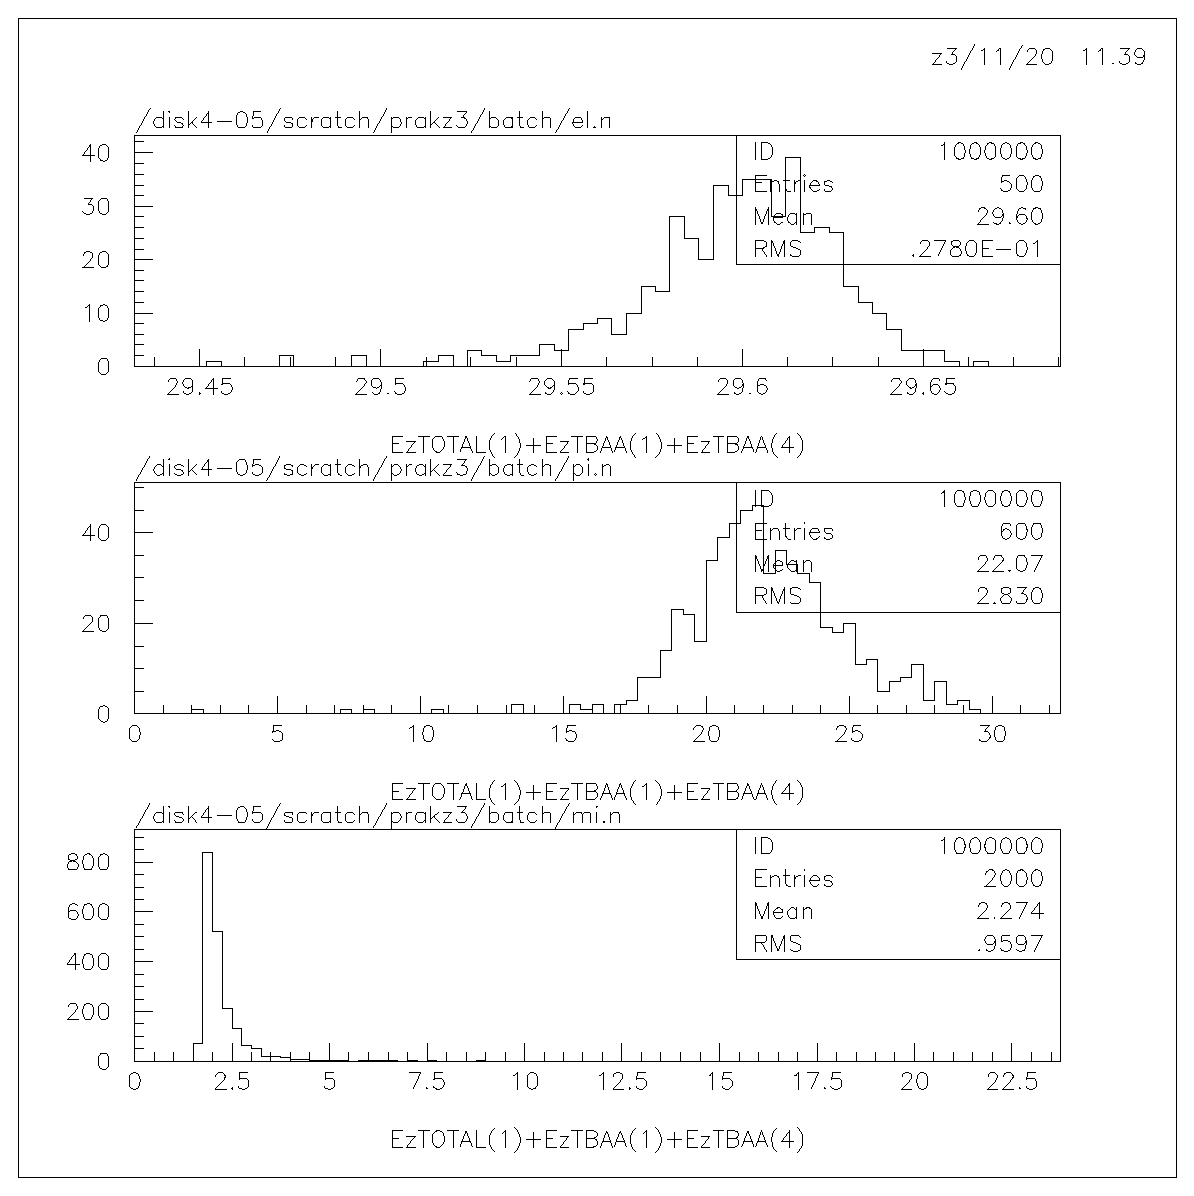
\includegraphics[scale=0.8]{data/pulmann_batch_crop.eps}
\caption{ Uložená energia v detektore \label{graph:batch}}
\end{graph}

\begin{figure}
        \centering
        \begin{subfigure}[b]{0.5\textwidth}
                \includegraphics[width=\textwidth]{output/sprska1crop.pdf}
                \caption{$\;e^-\; 10\unit{GeV}$}
                \label{fig:s1}
        \end{subfigure}%
        ~ 
        \begin{subfigure}[b]{0.5\textwidth}
                \includegraphics[width=\textwidth]{output/sprska2crop.pdf}
                \caption{$\;\gamma^-\; 100\unit{GeV}$}
                \label{fig:s2}
        \end{subfigure}
        \begin{subfigure}[b]{0.5\textwidth}
                \includegraphics[width=\textwidth]{output/sprska3crop.pdf}
                \caption{$\;\mu^-\; 10\unit{GeV}$}
                \label{fig:s3}
        \end{subfigure}%
        ~ 
        \begin{subfigure}[b]{0.5\textwidth}
                \includegraphics[width=\textwidth]{output/sprska4crop.pdf}
                \caption{$\;\mu^-\; 1\unit{GeV}$}
                \label{fig:s4}
        \end{subfigure}
        \begin{subfigure}[b]{0.5\textwidth}
                \includegraphics[width=\textwidth]{output/sprska5crop.pdf}
                \caption{$\;\mu^-\; 10\unit{TeV}$}
                \label{fig:s5}
        \end{subfigure}%
        ~ 
        \begin{subfigure}[b]{0.5\textwidth}
                \includegraphics[width=\textwidth]{output/sprska6crop.pdf}
                \caption{$\;\pi^0; 10\unit{GeV}$}
                \label{fig:s6}
        \end{subfigure}
\end{figure}

\begin{figure}
\ContinuedFloat
        
        \begin{subfigure}[b]{0.5\textwidth}
                \includegraphics[width=\textwidth]{output/sprska7crop.pdf}
                \caption{$\;\pi^+\; 100\unit{GeV}$}
                \label{fig:s7}
        \end{subfigure}%
        ~ 
        \begin{subfigure}[b]{0.5\textwidth}
                \includegraphics[width=\textwidth]{output/sprska8crop.pdf}
                \caption{$\;\pi^+\; 10\unit{GeV}$}
                \label{fig:s8}
        \end{subfigure}
        
        \begin{subfigure}[b]{0.5\textwidth}
                \includegraphics[width=\textwidth]{output/sprska9crop.pdf}
                \caption{$\;n\; 10\unit{GeV}$}
                \label{fig:s9}
        \end{subfigure}
        \caption{Vzorové spŕšky}\label{fig:sprsky}
\end{figure}

Výstup interaktívnej analýzy, zaujímavé spektrá, sú v obrázku \ref{fig:sprsky}. Pod obrázkami sú nalietavajúce častice a ich energie, interakcie si ale zaslúžia ďalší komentár:
\begin{itemize}
\item \textbf{\ref{fig:s1}:} Vidíme elektromagnetickú spŕšku, kvôli nižšej energii elektrónu je relatívne malá. Na pravom konci je pozorovateľné stopa častice - takéto stopy nepozorujeme v prípade $\gamma$. Vidíme tiež, že elektrón interaguje už pred detektorom a okamžite po vstupe do detektora.
\item \textbf{\ref{fig:s2}:} Opäť ide o elektromagnetickú spŕšku. Je väčšia ako u elektrónu kvôli väčšej energii $\gamma$ fotónu. Fotón opäť reaguje takmer okamžite po vstupe do detektora, no pretože je nenabitý, pred ním ho nedetekujeme.
\item \textbf{\ref{fig:s3}:} Mión má dostatočnú energiu na to, aby preletel a zhodou náhod nevyvolal žiadnu pozorovateľnú spŕšku. Napriek tomu interagoval, vidíme, že  je jeho dráha vychýlená od pôvodného smeru. Zelená stopa vo všeobecnosti označuje ionizujúcu časticu.
\item \textbf{\ref{fig:s4}:} Mión s polovicou potrebnej energie na prekonanie dvoch metrov detektora zastal, ako sme očakávali, v polovici. Vidíme, že pred zastavením spustil pozorovateľnú elektromagnetickú spŕšku.
\item \textbf{\ref{fig:s5}:} Mión s obrovskou energiou vyvolá radu elektromagnetických spŕšok počas svojej cesty detektorom a na materiále za detektorom sa mu podarí vyraziť nejaké atómy, čím vyvolá prúd nabitých častíc.
\item \textbf{\ref{fig:s6}:} Neutrálny pión sa takmer vždy a takmer okamžite rozpadá na dva $\gamma$ fotóny. Tie vyvolali dve slabšie elektromagnetické spŕšky. Ide o ďalšiu z nenabitých častíc, preto nepozorujeme jej stopu pred detektorom
\item \textbf{\ref{fig:s7}:} Na obrázku je dobrý prípad zmiešanej hadrónovej spŕšky. Nalietavajúci kladný pión odovzdáva väčšinu energie rôznym hadrónom (čiary) a tiež nabitým časticam (+brzdné žiarenie). Niektoré častice ušli z detektora, zrejme ide o únik cez medzery v postranných, starších detektoroch.
\item \textbf{\ref{fig:s8}:} Vidíme že pri nižšej energii dostávame čistejšiu zrážku, vytvorené hadróny sú pomalšie. Jeden z nich prenikol do postranného detektoru a tam skončil.
\item \textbf{\ref{fig:s9}:} Posledná spŕška je zase pomerne čistá hadrónová. Nevidíme tu stopu častice, pretože išlo o neutrálny neutrón. Všetky tri predchádzajúce častice, interagujúce silnou interakciou, sa typicky dostali oveľa ďalej do detektoru ako ľahké častice vyvolávajúce elektromagnetickú spŕšku.
\end{itemize}
%%%
\section*{Diskusia}
Diskusia o interakciách a ich špecifikách prebehla hlavne vo výsledkoch merania. Boli sme schopný kvalitatívne popísať javy, ktoré sme pozorovali na simulácii. Medzi zaujímavé pozorovania patrí napríklad, že nie sme veľmi schopní rozlíšiť nabité pióny a protón (preto aj nie je záznam interakcie protónu v obrázku \ref{fig:sprsky}, vyzerá rovnako), napriek rozdielom v hmotnostiach. Obe tieto častice totiž interagujú s pomerne oveľa ťažšími jadrami. Naopak elektrón a mión (medzi ktorými aj je väčší relatívny rozdiel hmotností) reagujú na elektrónoch. Preto elektrón zastaví takmer okamžite a mión reaguje veľmi slabo - pri zrážkach s ľahkými elektrónmi neodovzdáva takú časť vlastnej energie. 

Pri interaktívnej spŕške by bolo zaujímavé mať možnosť nejakých spôsobom spusiť veľké množstvo interakcií a sledovať len niektoré špeciálne - napríklad mióny zanechávajúce veľké množstvo energie. Tak by sme mohli pozorovať aj spŕšky, ktoré sme kvôli ich malej pravdepodobnosti nepozorovali.

V grafe \ref{graph:batch} sa zase potvrdili predpoklady o spôsoboch interakcie - elektróny odovzdávajú prakticky celú energiu, u piónov sa nejaká časť stráca (popísané v teórii) a u miónov ide o pevnú hodnotu okolo $2\unit{GeV}$, s niekoľkými výnimočnými silnejšími interakciami. Z tvaru nameraných rozdelení môžeme usudzovať, že sme merali dostatočný počet interakcií - ich tvar sa dá dobre posúdiť. Rovnako aj pomer energie uloženej v scintilátore a celkovej energie mal už pomerne dobre definovaný priebeh. Boli by sme teda z výsledkov simulácie schopný určiť korekcie na energie častíc v závislosti na zachytenej energii.
%%%
\section*{Záver}
Spustili sme batch simuláciu pre pióny, mióny a elektróny a porovnali sme histogramy uložených energií v grafe \ref{graph:batch}. Pozorovali sme spŕšky rôznych častíc, naučili sme sa ich rozlišovať a popísať dôvody, prečo ich spŕšky majú dané vlastnosti. V obrázku \ref{fig:sprsky} sme uviedli spŕšky vybraných častíc a popísali sme tieto spŕšky (viz. výsledky merania).
%%%

\begin{thebibliography}{9}

\bibitem{stud}
    \emph{Stránky s pokynmi ku úlohe A6} \\
    \url{http://physics.mff.cuni.cz/vyuka/zfp/_media/zadani/texty/txt_406.pdf} 20.11.2013

\bibitem{showers}
    Particle shower. \textit{Wikipedia}
    \url{http://en.wikipedia.org/wiki/Particle_shower} 20.11.2013
    
\end{thebibliography}
\end{document}
